% ::setlocal makeprg=cd\ latex\ &&\ pdflatex\ -interaction=batchmode\ main.tex\ &&\ xdg-open\ main.pdf\ &&\ exit

\textit{The content of this chapter is mostly based on
\fullcite[ch. 9]{hartle2021gravity} and \fullcite[ch. 12]{shapiro2008black}.}


\section{Notation and Formalism}
\label{cap1:ssec:notation}

In the \textit{flat spacetime} we can introduce a coordinate basis for
four-vectors
\begin{equation}
    \mathbf{e_t} = (1,0,0,0), \quad
    \mathbf{e_y} = (0,1,0,0), \quad
    \mathbf{e_y} = (0,0,1,0), \quad
    \mathbf{e_z} = (0,0,0,1).
    \label{cap1:eq:coord_base}
\end{equation}
The set 
$\{ \mathbf{e_t}, \mathbf{e_x}, \mathbf{e_y}, \mathbf{e_z} \}$, is often
referred to as $\{ \mathbf{e_0}, \mathbf{e_1}, \mathbf{e_2}, \mathbf{e_3} \}$.
Any four-vector $\textbf{a}$ can then be written as

\begin{equation}
    \textbf{a}
    = a^t \mathbf{e_t} + a^x \mathbf{e_x} + a^y \mathbf{e_y} + a^z \mathbf{e_z}
    = a^0 \mathbf{e_0} + a^1 \mathbf{e_1} + a^2 \mathbf{e_2} + a^3 \mathbf{e_3}
    \label{cap1:eq:a}
\end{equation}

where $(a_t,~a_x,~a_y,~a_z)$, or equivalently $(a_0,~a_1,~a_2,~a_3)$, are the
components of the four-vector.

Another useful convention is to use Roman letters (usually $i$ or $j$) to refer
to indices 1, 2, 3 and Greek letters (usually $\mu$ or $\nu$) to refer to
indices 0, 1, 2, 3.
Using Einstein notation the expression in eq. \ref{cap1:eq:a}, can be rewritten
simply as $\textbf{a} = a^\mu \mathbf {e_\mu}$.
Other useful ways to specify the components of $\textbf{a}$ are

\begin{equation*}
    a^\mu = (a^t, a^x, a^y, a^z) \quad a^\mu = (a^t, a^i) \quad a^\mu
    = (a^t, \vec a)
\end{equation*}

where $\vec a = a^i e_i$ is the tree-dimensional vector $(a_x, a_y, a_z)$.

The length of the four-vector $\mathbf{a}$ must be evaluated using the line
element of the flat spacetime, described in eq. \ref{eq:Minkowski}.
In general, a useful way to do that is by first defining the \textit{metric}
$\eta_{\nu \mu}$

\begin{equation}
    \eta_{\nu \mu} = 
    \begin{array}{cc}
        \begin{pNiceMatrix}[first-row,first-col][columns-width = auto]
              & t & x & y & z \\
            t~~ & -1 & 0 & 0 & 0 \\  
            x~~ & 0 & 1 & 0 & 0 \\ 
            y~~ & 0 & 0 & 1 & 0 \\
            z~~ & 0 & 0 & 0 & 1 \\
        \end{pNiceMatrix} &
    \end{array}
    \quad \implies \quad
    \mathrm{d}s^2 = \eta_{\nu \mu} \mathrm{d}x^\nu \mathrm{d}x^\mu
\end{equation}

Here the double sum is implied, and we rightfully notice that the minus sign has
appeared again under the $t$ component.
Now we can compactly write

\begin{equation}
    \mathbf{a} \cdot \mathbf{a} = \eta_{\mu \nu} \, a^\mu \, a^\nu
    = - (a^t)^2 + (a^x)^2 + (a^y)^2 + (a^z)^2
\end{equation}

Without any claim of rigorously demonstrating it, we can say that since this
scalar product is built from the line element $\mathrm{d}s^2$, it is the same
in every inertial frame one might choose. Quantities that have these properties
are \textit{invariant}.

When working in the \Sh geometry it is useful to adopt the \Sh coordinates:
spherical coordinates centered at the center of the mass $M$.
Instead of describing a four-vector with the components $(a_t,~a_x,~a_y,~a_z)$,
we will use $(a_t,~a_r,~a_\theta,~a_\phi)$.

Given the expression of the line element in eq. \ref{eq:Sh} it is useful to
adopt geometrized units, where $G = c = 1$
(Appendix \ref{ap:geometrized_units}).
From now on we will always use geometrized units (referring to them as
$\mathcal L$) unless stated otherwise.
The line element and the metric can be rewritten as

\begin{equation}
    \mathrm{d}s^2 = - \left(1 - \frac{2 M}{r} \right) (\mathrm{d}t)^2
    + \left(1 - \frac{2 M}{r} \right)^{-1} \mathrm{d}r^2
    + r^2 (\mathrm{d}\theta^2 + \sin^2 \theta \mathrm{d}\phi^2)
    \label{cap1:eq:Sh_ds1}
\end{equation}

\begin{equation}
    g_{\nu \mu} = 
    \begin{array}{cc}
        \begin{pNiceMatrix}[first-row,first-col][columns-width = auto]
              & t & r & \theta & \phi \\
            t~~ & - (1 - 2 M /r) & 0 & 0 & 0 \\  
            r~~ & 0 & (1 - 2 M /r)^{-1} & 0 & 0 \\ 
            \theta~~ & 0 & 0 & r^2 & 0 \\
            \phi~~ & 0 & 0 & 0 & r^2 \sin^2 \theta \\
        \end{pNiceMatrix} &
    \end{array}
    .
    \label{cap1:eq:Sh_g}
\end{equation}

It is worth pointing out that, given \ref{cap1:eq:Sh_ds1} and
\ref{cap1:eq:Sh_g}, when we introduce this coordinate frame 

\begin{equation}
    \mathbf{e_t} = (1,~0,~0,~0) \quad
    \mathbf{e_r} = (0,~1,~0,~0) \quad
    \mathbf{e_\theta} = (0,~0,~1,~0) \quad
    \mathbf{e_\phi} = (0,~0,~0,~1)
\end{equation}

it has the inconvenience of not being normalized. For example

\begin{equation}
    \mathbf{e_t \cdot e_t} = g_{\nu \mu} e_t^\mu e_t^\nu = g_{00}
    = - (1 - 2 M /r) \, .
\end{equation}

If we want an orthonormal tetrad we can define

\begin{subequations}
\begin{align}
    \mathbf{\hat e_t} &= \left(1 - \frac{2M}{r}\right)^{-1/2} \mathbf{e_t}
    \quad &&\implies \quad
    \mathbf{\hat e_t \cdot \hat e_t} = g_{\nu \mu} \hat e_t^\mu \hat e_t^\nu
    = g_{00} \left(1 - \frac{2M}{r}\right)^{-1} = - 1
    \label{cap1:eq:local_ON_base_t}\\
    %
    \mathbf{\hat e_r} &= \left(1 - \frac{2M}{r}\right)^{1/2} \mathbf{e_r}
    \quad &&\implies \quad
    \mathbf{\hat e_r \cdot \hat e_r} = g_{\nu \mu} \hat e_r^\mu \hat e_r^\nu
    = g_{00} \left(1 - \frac{2M}{r}\right) = 1 \\
    %
    \mathbf{\hat e_\theta} &= \frac{1}{r} \mathbf{e_t}
    \quad &&\implies \quad
    \mathbf{\hat e_\theta \cdot \hat e_\theta} = 1 \\
    %
    \mathbf{\hat e_\phi} &= \frac{1}{r \sin \theta} \mathbf{e_t}
    \quad &&\implies \quad
    \mathbf{\hat e_\phi \cdot \hat e_\phi} = 1
\end{align}
    \label{cap1:eq:local_ON_base}
\end{subequations}

\newpage


\section{Proprieties of the Metric}

Let's first analyze the \Sh metric in more detail:

\begin{equation}
    \mathrm{d}s^2 = - \left(1 - \frac{2 M}{r} \right) (\mathrm{d}t)^2
    + \left(1 - \frac{2 M}{r} \right)^{-1} \mathrm{d}r^2
    + r^2 (\mathrm{d}\theta^2 + \sin^2 \theta \mathrm{d}\phi^2)
    \label{cap1:eq:Sh_ds}
\end{equation}

There are two singularities in $r = 0$ and $r = 2M$.
The first one is a true, physical singularity, since the spacetime curvature
diverges for $r \rightarrow 0$.
The second one is a coordinate singularity and occurs at what is defined as the
\Sh $r_s = 2M$.
Every non-black hole object has a radius larger than its \Sh radius.
The nature and significance of this will become clearer in the subsequent
sections.

On the other hand, if we take the limit as $r$ approaches infinity, we notice
that the metric becomes asymptotically flat, approaching the metric of \Mi
space.
Therefore, we can refer to the value a quantity would have at a great distance
to find a more familiar expression.

Finally, $\mathrm{d}s^2$ is independent of the coordinates $t$ and $\phi$.
This is expected, as the mass responsible for curving the spacetime is static
and spherically symmetric or in the case of a black hole solution, the spacetime
is spherical and stationary (Birkhoff’s theorem guarantees that if the metric is
spherically symmetric and static, then it is also stationary).
The metric independence from time and rotation implies the existence of two,
easy to find, \textit{Killing vectors}:

\begin{equation}
    \xi = (1, 0, 0, 0) \quad \text{and} \quad \eta = (0, 0, 0, 1) \, .
    \label{cap1:eq:xi_eta}
\end{equation}

A \textit{killing vector} is a direction in the four-dimensional spacetime
along which we can freely move without changing the metric.
It is a general way to describe a symmetry of the metric.
Since symmetries correspond to conserved quantities they will be a key point in
studying the trajectories of free particles and photons.

We start by considering the four-momentum $\mathbf{p}$ of a particle of mass
$m$, defined as

\begin{equation}
    p^\mu := m u^\mu = m \dv{x^\mu}{\tau}
\end{equation}

where $u$ is the four-velocity of the particle, $x$ a four-vector describing its
position and $\tau$ the
proper time.
Therefore, for a free particle, the quantities

\begin{align*}
    E &= - \mathbf{\xi \cdot p} =
    - g_{00} \, p^0 = m \left( 1 - \frac{2M}{r} \right) \dv{x^t}{\tau} \\
    L &= \mathbf{\eta \cdot p} =
    g_{33} \, p^\phi = m r^2 \sin^2 \theta \dv{x^\phi}{\tau}
\end{align*}

will be conserved during the motion.
We already named them $E$ and $L$ as they are respectively the energy and the
angular momentum at large $r$ and low velocities.
To simplify the expressions used in the discussion will use normalized
quantities

\begin{subequations}
    \begin{align}
        e &:= \frac{E}{m} = \left( 1 - \frac{2M}{r} \right) \dv{x^t}{\tau}
        \label{cap1:eq:conserved_e} \\
        \ell &:= \frac{L}{m} = r^2 \sin^2 \theta \dv{x^\phi}{\tau} \, .
        \label{cap1:eq:conserved_l}
    \end{align}
\end{subequations}

$e$ and $\ell$ are respectively the conserved energy and angular momentum per
unit
rest mass.

For a massless particle (e.g. a photon) the proper time can not be used, so
the four-velocity can be defined using an \textit{affine parameter} $\lambda$.

\begin{equation}
    u^\mu = \dv{x^\mu}{\lambda}
    \label{cap1:eq:u_light}
\end{equation}

We can define the conserved quantities $e$ and $l$ in the same way, using the
four-velocity

\begin{subequations}
    \begin{align}
        e &:= - \xi \cdot \mathbf{u}
        = \left( 1 - \frac{2M}{r} \right) \dv{x^t}{\lambda} \\
        \ell &:= \eta \cdot \mathbf{u} 
        = r^2 \sin^2 \theta \dv{x^\phi}{\lambda} \, .
        \label{cap1:eq:e_light}
    \end{align}
    \label{cap1:eq:conserved_light}    
\end{subequations}

getting the same result except for having $\lambda$ instead of $\tau$.

In the next sections the normalization of the four-velocity $\mathbf u$ will be
really useful too

\begin{subequations}
    \begin{align}
        &\mathbf{u \cdot u} = g_{\nu \mu} u^\nu u^\mu = -1 
        &&\text{for } m \neq 0 \label{cap1:eq:u_normalization_mass} \\
        &\mathbf{u \cdot u} = g_{\nu \mu} u^\nu u^\mu = 0 
        &&\text{for } m = 0 \label{cap1:eq:u_normalization_light} \, .
    \end{align}
    \label{cap1:eq:u_normalization}
\end{subequations}

It is not just a property of the metric, but it is valid for every
$g_{\nu \mu}$.
Equations \ref{cap1:eq:u_normalization_mass} and
\ref{cap1:eq:u_normalization_light} can be respectively derived in this way:
\begin{subequations}
\begin{align}
    g_{\nu \mu} \mathrm{d}x^\nu \mathrm{d}x^\mu = \mathrm{d}s^2
    \quad &\implies \quad
    g_{\nu \mu} \dv{x^\nu}{\tau} \dv{x^\mu}{\tau} = \dv{s^2}{\tau^2}
    \quad &&\implies \quad
    \mathbf{u \cdot u} = -1 \label{cap1:eq:proof1} \\
    %
    g_{\nu \mu} \mathrm{d}x^\nu \mathrm{d}x^\mu = \mathrm{d}s^2
    \quad &\implies \quad
    g_{\nu \mu} \dv{x^\nu}{\lambda} \dv{x^\mu}{\lambda} = 0
    \quad &&\implies \quad
    \mathbf{u \cdot u} = 0 \label{cap1:eq:proof2}
\end{align}
\end{subequations}

Using the definition of proper time $\mathrm{d}\tau^2 = - \mathrm{d}s^2$ in
\ref{cap1:eq:proof1} and the property of the light rays $\mathrm{d}s^2 = 0$ in
\ref{cap1:eq:proof2}.


\section{Gravitational Redshift}

Let's consider a static observer in $r$.
When an observer measures the energy of a photon, that corresponds to the $t$
component of the four-momentum of the photon, $\mathbf{p}$,
%%% p?
they do that using their local orthonormal tetrad
that we described in \ref{cap1:eq:local_ON_base}.

Referring to $p^{\hat t}$ as the value measured in the orthonormal tetrad
$\{ \mathbf{\hat e_t, \hat e_r, \hat e_\theta, \hat e_\phi} \}$ and
$p^t$ as the value measured with the coordinate basis
$\{ \mathbf{e_{t}, e_{r}, e_{\theta}, e_{\phi}} \}$, the energy measured in $r$ will be

\begin{equation*}
    E(r) = p^{\hat t} = \mathbf{p \cdot \hat e_t}
    = \mathbf{p \cdot e_t} \left(1 - \frac{2M}{r} \right)^{-1/2}
    = \mathbf{p \cdot \xi} \left(1 - \frac{2M}{r} \right)^{-1/2}
\end{equation*}
\begin{equation}
    \left(1 - \frac{2M}{r} \right)^{1/2} E(r) = \mathbf{p \cdot \xi}
    = \text{const} \, .
    \label{cap1:eq:photon_energy1}
\end{equation}

Where we used the expression for $\hat e_t$ from eq.
\ref{cap1:eq:local_ON_base_t}
and notice that $\mathbf{e_t} = \xi$ from eq. \ref{cap1:eq:coord_base} and eq.
\ref{cap1:eq:xi_eta}. 
Solving for the constant $\mathbf{p} \cdot \xi$ we find the expression in
\ref{cap1:eq:photon_energy1}. The relationship between the energy of a photon
measured at $r'$ and the one measured at $r$ from two static observers using
their own tetrad is

\begin{equation*}
    \left(1 - \frac{2M}{r'} \right)^{1/2} E(r')
    = \left(1 - \frac{2M}{r} \right)^{1/2} E(r)
\end{equation*}

Taking the limit as $r'$ approaches infinity and using $E = \hbar \omega$ for
the energy of the photon

\begin{equation}
    \omega_\infty = \omega_* \left(1 - \frac{2M}{r} \right)^{1/2} \, .
    \label{cap1:eq:redshift}
\end{equation}

Here, $\omega_\infty$ is the frequency measured by a distant observer at
$r \gg r_s$, while $w_*$ denotes the frequency measured at a specific distance
$r$.
Photons observed at a certain distance from a star exhibit a lower frequency
compared to the one they have at the point of emission.


\section{Particle Orbits}
\label{cap1:sec:particle_orbits}

\begin{minipage}{0.4 \textwidth}

% 3D AXIS with spherical coordinates
\tdplotsetmaincoords{60}{110}
\begin{tikzpicture}[scale=2,tdplot_main_coords]
  
    % Red vector coordinates
    \def\rvec{1.15}
    \def\thetavec{90}
    \def\phivec{70}
    
    % AXES
    \coordinate (O) at (0,0,0);
    \draw[thick,->] (0,0,0) -- (2,0,0) node[right=1]{$x$};
    \draw[thick,->] (0,0,0) -- (0,2,0) node[above=1]{$y$};
    \draw[thick,->] (0,0,0) -- (0,0,2) node[left=1]{$z$};
    
    % VECTORS
    \tdplotsetcoord{P}{\rvec}{\thetavec}{\phivec}
    \draw[thick,red] (O)  -- (P) node[below right]
        {$(r, \theta = \frac{\pi}{2}, \phi)$};
    %\draw[dashed]   (O)  -- (Pxy);
    \draw[dashed]   (P)  -- (Pxy);
    
    % ARCS
    \tdplotdrawarc[thick,->]{(O)}{0.4}{0}{\phivec} {anchor=north}{$\phi$}
    \tdplotsetthetaplanecoords{\phivec}
    \tdplotdrawarc[thick,->,tdplot_rotated_coords]{(0,0,0)}{0.5}{0}{\thetavec}
        {anchor=south west}{\hspace{-1mm}$\theta$}

    % Particle trajectory in XY plane
    \draw[thick,green,domain=-1.5:1.8,samples=100,variable=\t] 
        plot (\t, {1.5 - 1/(\t + 2)}, 0);
    % Dashed at the beginning
    \draw[thick,green,dashed,domain=1.8:2.3,samples=100,variable=\t] 
        plot (\t, {1.5 - 1/(\t + 2)}, 0);
    % Dashed at the end
    \draw[thick,green,dashed,domain=-1.55:-1.52,samples=100,variable=\t] 
        plot (\t, {1.5 - 1/(\t + 2)}, 0);

    % Center Point
    \shade[inner color=white, outer color=blue!60!black] (0,0,0) circle (3pt);

\end{tikzpicture}
\captionof{figure}{Visual representation of the spherical coordinates used.
The green line represents a possible trajectory on the $xy$ plane. \\}
\label{cap1:fig:spherical_coordinates}
\end{minipage}
\hspace{0.02 \textwidth}
\begin{minipage}{0.57 \textwidth}
    To further analyze the \Sh geometry, we will now explore the behavior of a
    test particle within it.
    The term \textit{test particle} refers to an object with mass so small that
    its influence on the surrounding spacetime is negligible, allowing us to
    analyze its motion without altering the geometry of the spacetime itself.

    As already established from eq. \ref{cap1:eq:conserved_l} the angular
    momentum is conserved during the motion of a particle in this geometry.
    This implies that the particle's orbit must lie within a plane.
    Without loosing generality we can imagine the particle path to stay in the
    $xy$ plane, fixing $\theta = \pi / 2$ and, consequently,
    \begin{equation*}
        u^\theta = \dv{\theta}{\tau} = 0 
    \end{equation*}
    \begin{equation*}
        \ell = r^2 \sin^2 \theta \dv{\phi}{\tau} = r^2 \dv{\phi}{\tau}
    \end{equation*}

    Refer to Figure \ref{cap1:fig:spherical_coordinates} for a visual
    representation.
\end{minipage}
\hspace{0.02 \textwidth}

The four-velocity of our test particle can then be written as
\begin{equation*}
    u^\mu
    = \left(\dv{x^t}{\tau},~\dv{x^r}{\tau},~\dv{x^\theta}{\tau},~
    \dv{x^\phi}{\tau} \right)
    = \left(e \left(1 - \frac{2M}{r}\right)^{-1},~\dv{r}{\tau},~0,~
    \frac{\ell}{r^2} \right) \, .
\end{equation*}

Where we simplified the notation using $r = x^r$ and eliminated
the dependence from $x^t$ and $x^\phi$ using the conserved quantities $e$ (eq.
\ref{cap1:eq:conserved_e}) and $\ell$ (eq. \ref{cap1:eq:conserved_l})
respectively.
Thanks to the normalization of $\mathbf u$ (eq.
\ref{cap1:eq:u_normalization_mass}) and using $\theta = \pi / 2$ again, we can
write

\begin{equation*}
    - 1 = g_{\nu \mu} u^\nu u^\mu =
    - \left(1 - \frac{2M}{r} \right)^{-1} e^2
    + \left(1 - \frac{2M}{r} \right)^{- 1} \left(\dv{r}{\tau} \right)^2
    + \frac{\ell^2}{r^2} \, .
\end{equation*}

Rearranging the expression, we have

\begin{equation}
    e^2 = \left(\dv{r}{\tau}\right)^2 + \left(1 + \frac{\ell^2}{r^2}\right)
    \left(1 - \frac{2M}{r} \right) \, .
   \label{cap1:eq:found_e}
\end{equation}

To compare eq. \ref{cap1:eq:found_e} with the Newtonian case we can expand
the product, subtract 1 from both sides and divide by a factor of 2:

\begin{equation}
    \mathcal E := \frac{e^2 - 1}{2} = \frac{1}{2} \left(\dv{r}{\tau}\right)^2
    + \frac{\ell^2}{2 r^2} - \frac{M}{r} - \frac{M \ell^2}{r^3} \, .
    \label{cap1:eq:found_epsilon}
\end{equation}

By defining this dimensionless constant $\mathcal E$, we can now see the
derivative of $r$ as the kinetic energy (per unit rest mass) and the other
terms as an effective potential acting on the particle, defined as

\begin{equation}
    V_{\rm eff}(r)
    := \frac{\ell^2}{2 r^2} - \frac{M}{r} - \frac{M \ell^2}{r^3} \, .
    \label{cap1:eq:V_eff}
\end{equation}

To better understand eq. \ref{cap1:eq:V_eff}, we can express it in
$\mathcal{LMT}$ units, substituting $\ell \rightarrow \ell / c$ and 
$ M \rightarrow G M / c^2$

\begin{equation*}
    V_{\rm eff}(r)
    = \frac{1}{c^2} \left( \frac{\ell^2}{2 r^2} - \frac{G M}{r}
    - \frac{G M \ell^2}{c^2 r^3} \right)
\end{equation*}
The first two terms are identical to the Newtonian potential for a particle
with angular momentum (per mass) $\ell$, orbiting around an object of mass $M$.
The third one is new, negligible for $GM\ell^2 \ll c^2 r^3$, and it is
proportional
to $r^{-3}$.

Figure \ref{cap1:fig:V_effvsVN} shows the effect of the $r^{-3}$ term: the
infinite centrifugal barrier of the Newtonian potential disappears in
$V_{\rm eff}$ and a particle with enough energy can fall to the center of the
massive object.

\begin{figure}[h]
\begin{minipage}{0.49 \textwidth}
    \centering
    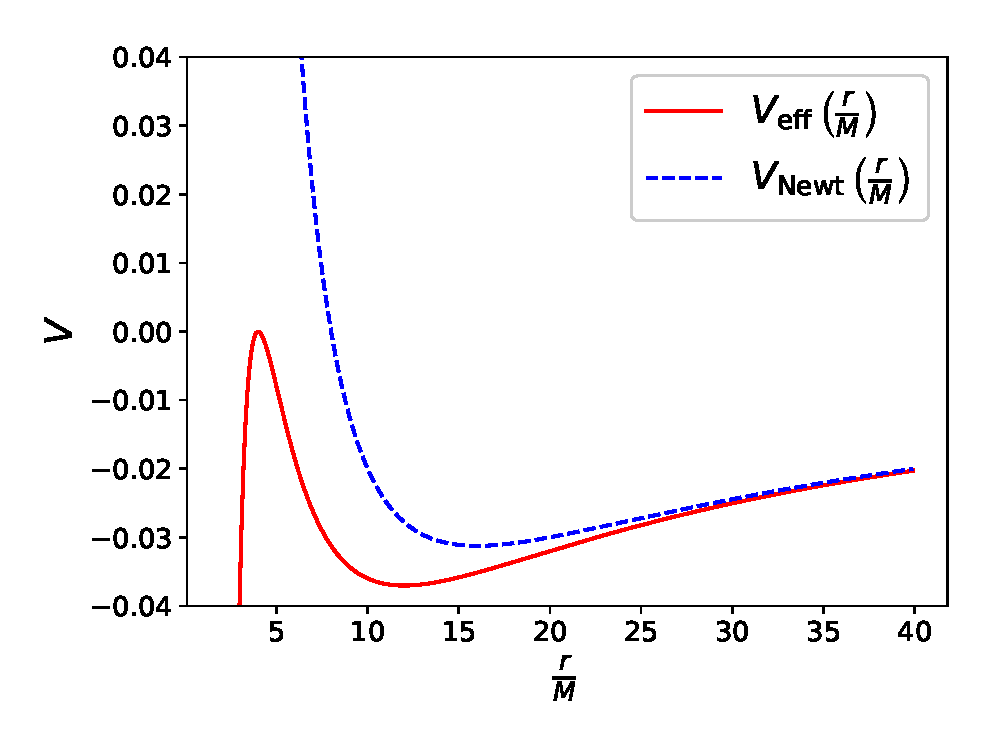
\includegraphics[width = \textwidth]{Figures/chapter1/V_eff.eps}
    \caption{Effective potential defined in eq. \ref{cap1:eq:V_eff} against the
    Newtonian potential, $\ell / M = 4$. \\
    The $r^{-3}$ term dominates for $r \sim r_s$ and the
    particle can fall into the massive object.
    On the other hand the Newtonian potential presents its characteristic
    infinite centrifugal barrier.}
    \label{cap1:fig:V_effvsVN}
\end{minipage}
\hspace{0.009 \textwidth}
\begin{minipage}{0.49 \textwidth}
    \centering
    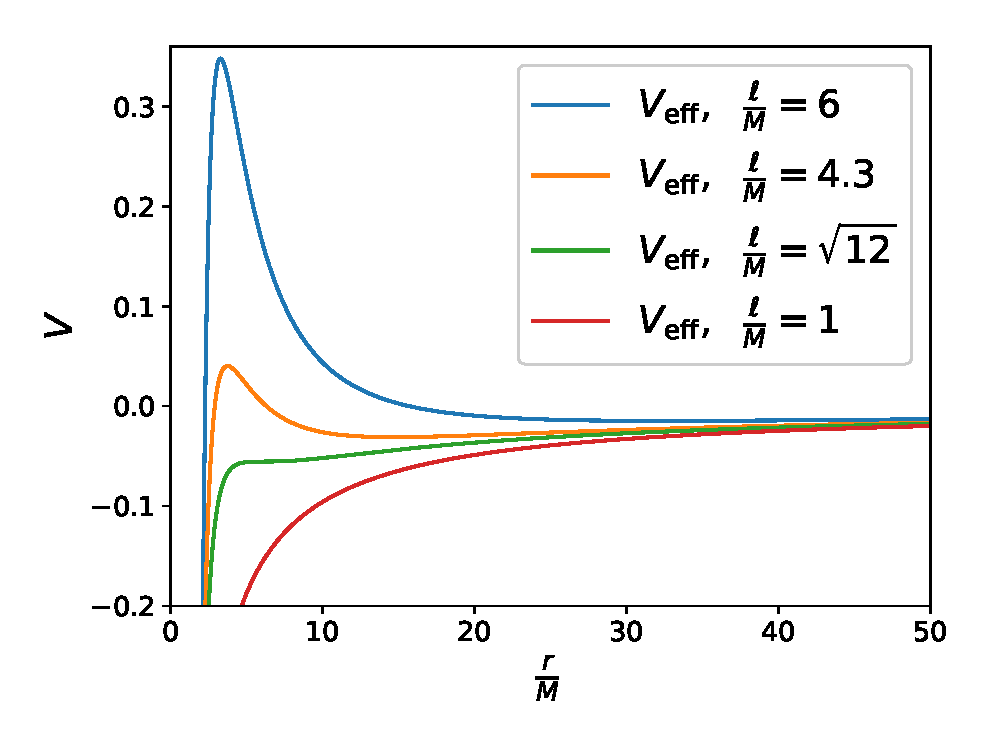
\includegraphics[width = \textwidth]{Figures/chapter1/V_eff_tanti.eps}
    \caption{$V_{\rm eff}$ for different values of $\ell / M$.
    For $\ell / M = \sqrt{12}$ (green) we can see $r_{\rm ISCO}$
    the limit of the smallest stable orbit (eq. \ref{cap1:eq:r_ISCO}.
    For $\ell / M = 1$ (red) there is no stationary point.
    The only stable points can be found for $\ell / M > \sqrt{12}$,
    in $r_{\rm min}$, defined in eq. \ref{cap1:eq:r_min_max}.}
    \label{cap1:fig:V_eff_tanti}
\end{minipage}
\end{figure}

By Taking the derivative of $V_{\rm eff}$ with respect to $r$ we can predict the
existence of stationary points for $\frac{\ell}{M} \geq \sqrt{12}$.

\begin{subequations}
\begin{align}
    r_{\substack{\rm max \\ \rm min}} &= \frac{\ell^2}{2 M} \left[1 \pm
    \sqrt{1 - 12 \left( \frac{M}{\ell} \right)^2} \, \right]
    &&\frac{\ell}{M} > \sqrt{12} \label{cap1:eq:r_min_max} \\
    %
    r_{\rm ISCO} &= 6 M
    &&\frac{\ell}{M} = \sqrt{12} \label{cap1:eq:r_ISCO}
\end{align}
\label{cap1:eq:stationary_r}
\end{subequations}

In eq. \ref{cap1:eq:r_min_max} $r_{\rm max}$ and $r_{\rm min}$ correspond
to an unstable point and to a stable one respectively.

The case described by eq. \ref{cap1:eq:r_ISCO} represents the
\textit{innermost stable circular orbit} (ISCO).
As the name suggests, it is the limit of the smallest stable orbit that a
particle can theoretically follow.
It is shown in green in Figure \ref{cap1:fig:V_eff_tanti}.

For $\frac{\ell}{M} < \sqrt{12}$ there are no stationary points and the particle
either escapes to infinity or falls towards the mass $M$ (red line in Figure
\ref{cap1:fig:V_eff_tanti}).

As in the Newtonian case a bound orbit exists only when $V_{\rm eff}$ has a
stable stationary point and the total energy given to the particle is not
greater than $V_{\rm eff}(r_{\rm max})$ (a more detailed explanation will be given in
Section \ref{cap1:sec:stable_orbits}).


\section{The Simplest Geodesics: Radial Infalls}

The simplest case of particle we can consider is a radial infall where $\phi$
stays constant.
From eq. \ref{cap1:eq:conserved_l} this implies $\ell = 0$.

Eq. \ref{cap1:eq:found_e} becomes


\begin{equation*}
    e^2 = \left(\dv{r}{\tau}\right)^2 + 1 - \frac{2M}{r}
\end{equation*}
\begin{equation}
    \dv{r}{\tau} = - \sqrt{e^2 - 1 + \frac{2 M}{r}} \, .
    \label{cap1:eq:radial_infall_ODE_1}
\end{equation}

Where we chose the negative root as we want to discuss the case where the radius
is decreasing.
Looking at the parameter $e$ in eq. \ref{cap1:eq:radial_infall_ODE_1} we can
distinguish 3 cases:

\begin{itemize}
    \item $e^2 < 1$: the particle has to start from a finite radius $r = R$
        for the argument of the square root to be positive;
    \item $e = 1$: the particle starts at rest from $r = \infty$ (that implies
        $\dv{t}{\tau} = 1$ at infinity and $e = 1$ from eq.
        \ref{cap1:eq:conserved_e});
    \item $e^2 > 1$: the particle starts from $r = \infty$ and also has some
        inward velocity.
\end{itemize}

We choose to analyze the case where $e = 1$ because it allows to easily solve
eq. \ref{cap1:eq:radial_infall_ODE_1} analytically.
We get

\begin{equation}
    \dv{r}{\tau} = - \sqrt{\frac{2 M}{r}} \, .
    \label{cap1:eq:radial_infall_ODE_2}
\end{equation}
\begin{equation*}
    r^{1/2} \mathrm{d}r = -(2M)^{1/2} \mathrm{d}\tau
\end{equation*}
\begin{equation}
    r(\tau) = \left(\frac{3}{2}\right)^{2/3}
    (2M)^{1/3} (\tau_* - \tau)^{2/3} \, .
    \label{cap1:eq:radial_infall_r_of_tau}
\end{equation}

Where $\tau_*$ is an integration constant that fixes the proper time $\tau$
when the particle arrives at $r = 0$.
An observer that falls together with the particle will measure a finite time
when he reaches $r = 2M$ and $\tau = \tau_*$ at $r = 0$.

On the contrary the experience of an observer far away from the source of
curvature, that measures the \Sh time $t$ it is much different.
To see this we can solve eq. \ref{cap1:eq:radial_infall_ODE_2} with respect to
$t$.
Using the chain rule to derive $r$ with respect to $t$ and eliminating the
dependence from $\tau$ using eq. \ref{cap1:eq:conserved_e} with $e = 1$, we get

\begin{align*}
    - \sqrt{\frac{2 M}{r}} = \dv{r}{\tau} = \dv{t}{\tau} \dv{r}{t}
    = \left(1 - \frac{2M}{r} \right)^{-1} \dv{r}{t}
\end{align*}
\begin{equation*}
    \dv{t}{r} = - \left(\frac{2 M}{r}\right)^{-1/2}
    \left(1 - \frac{2M}{r} \right)^{-1} \,  \, 
\end{equation*}

The integration is not as immediate as the previous one, but can be resolved
by substituting $u = \sqrt{r}$ and then by breaking the fraction into simpler
ones repeatedly.
The result, fixing a similar time constant $t_*$ as before, is

\begin{equation}
    t = t_* + 2M \left[ -\frac{3}{2} \left(\frac{r}{2M}\right)^{3/2}
    - 2 \left(\frac{r}{2M}\right)^{1/2}
    + \ln \abs{\frac{(r/2M)^{1/2} + 1}{(r/2M)^{1/2} - 1}} \right] \, .
    \label{cap1:eq:radial_infall_r_of_t}
\end{equation}

We can not find $r(t)$ analytically as was done previously, but the expression
in \ref{cap1:eq:radial_infall_r_of_t} already tells us that for
$r \rightarrow 2M$ the time measured by a far observer goes to infinity.
This implies that the distant observer will never see the particle reaching
$r = 2M$ and entering the \Sh radius, they will only see it getting closer and
closer forever. \\
If the particle is emitting a signal with a frequency $w_*$, they will measure
it infinitely redshifted as described by eq. \ref{cap1:eq:redshift},
asymptotically going to $\omega_\infty = 0$.
That is why the \Sh radius is also referred to as a
\textit{source of infinite redshift}. \\
Figure \ref{cap1:fig:radial_infall} shows eq.
\ref{cap1:eq:radial_infall_r_of_tau} and eq
\ref{cap1:eq:radial_infall_r_of_t}, the integration constants $\tau_*$ and
$t_*$ where chosen to make both equations start from the same point
$r \simeq 12M$ at $\tau = t =  0$.

\begin{figure}[h]
    \centering
    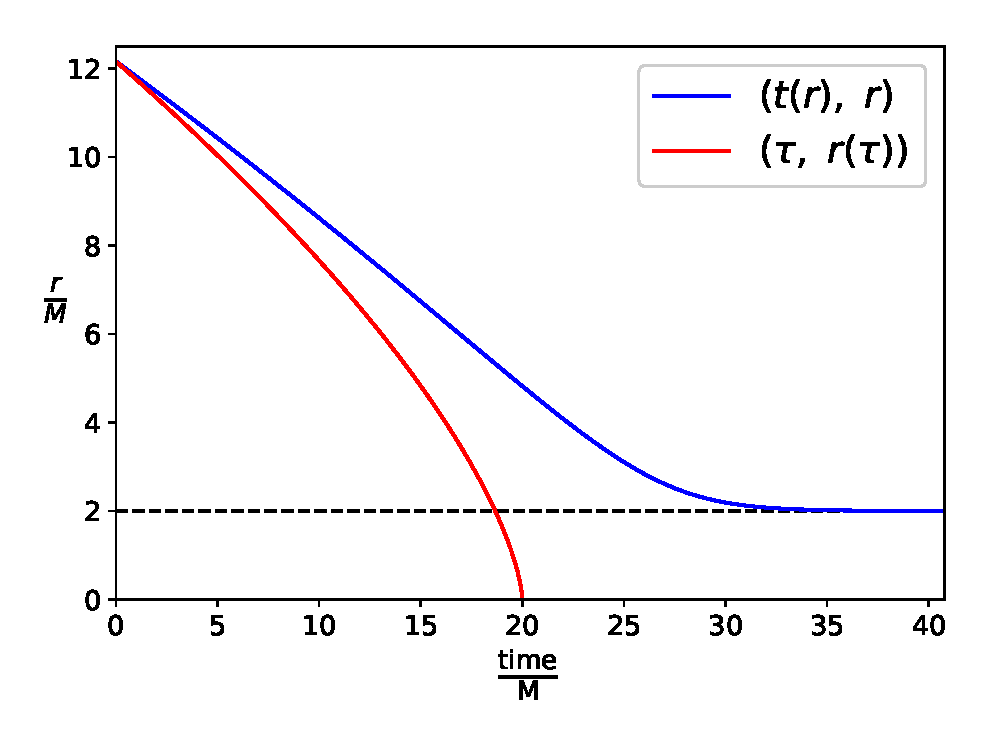
\includegraphics[width = 0.8 \textwidth]{Figures/chapter1/radial_infall.eps}
    \caption{Eq. \ref{cap1:eq:radial_infall_r_of_tau} and eq.
    \ref{cap1:eq:radial_infall_r_of_t} describing the fall from
    $r \simeq 12M$ on.
    The integration constants $\tau_*$ and $t_*$ where fixed so that both
    equations started from the same $r(0)$.
    $r(\tau)$ gets to 0 quickly (at $\tau = \tau_*$), while $t(r)$ goes to
    infinity for $r \rightarrow r_s = 2M$. The \Sh radius $r_s$ is represented
    with the dashed black line.}
    \label{cap1:fig:radial_infall}

    %% Va bene il grafico? credo potrebbe essere poco appropriato perché tempo 
     % proprio e tempo di \Sh dovrebbero essere uguali solo a r = \infty.
     % In teoria dovrei utilizzare l'equazione differenziale con e^2 < 1 in modo che
     % la particella parta da una distanza finita.
     % C'è il grafico fatto bene a pagina 344 del
     % Black Holes, White Dwarfs, and Neutron Stars (stuart L., Shapiro Saul A. Teukolsky)
     % che a sua volta è stato preso dal Gravitation Misner Thorne Wheeler 1973,
     % che ho trovato sull'Internet Archive
     % https://archive.org/details/GravitationMisnerThorneWheeler/page/n689/mode/2up
     % le 4 pagine sono in doc/
\end{figure}

\newpage


\section{Stable Orbits}
\label{cap1:sec:stable_orbits}

In Section \ref{cap1:sec:particle_orbits} we analyzed the role that
$\frac{\ell}{M}$ has on the effective potential $V_{\rm eff}$ defined in eq.
\ref{cap1:eq:V_eff} and found out that for $\frac{\ell}{M} > \sqrt{12}$ it has
two stationary points $r_{\substack{\rm max \\ \rm min}}$ defined in eq.
\ref{cap1:eq:r_min_max}.

For clarity, we rewrite eq. \ref{cap1:eq:found_epsilon} below, accompanied by a
visual representation in Figure \ref{cap1:fig:V_eff_orbits}.

\begin{equation}
    \left( \dv{r}{\tau} \right)^2 = \mathcal E - V_{\rm eff} (r)
    \label{cap1:eq:like_newton}
\end{equation}

\begin{figure}[h]
    \centering
    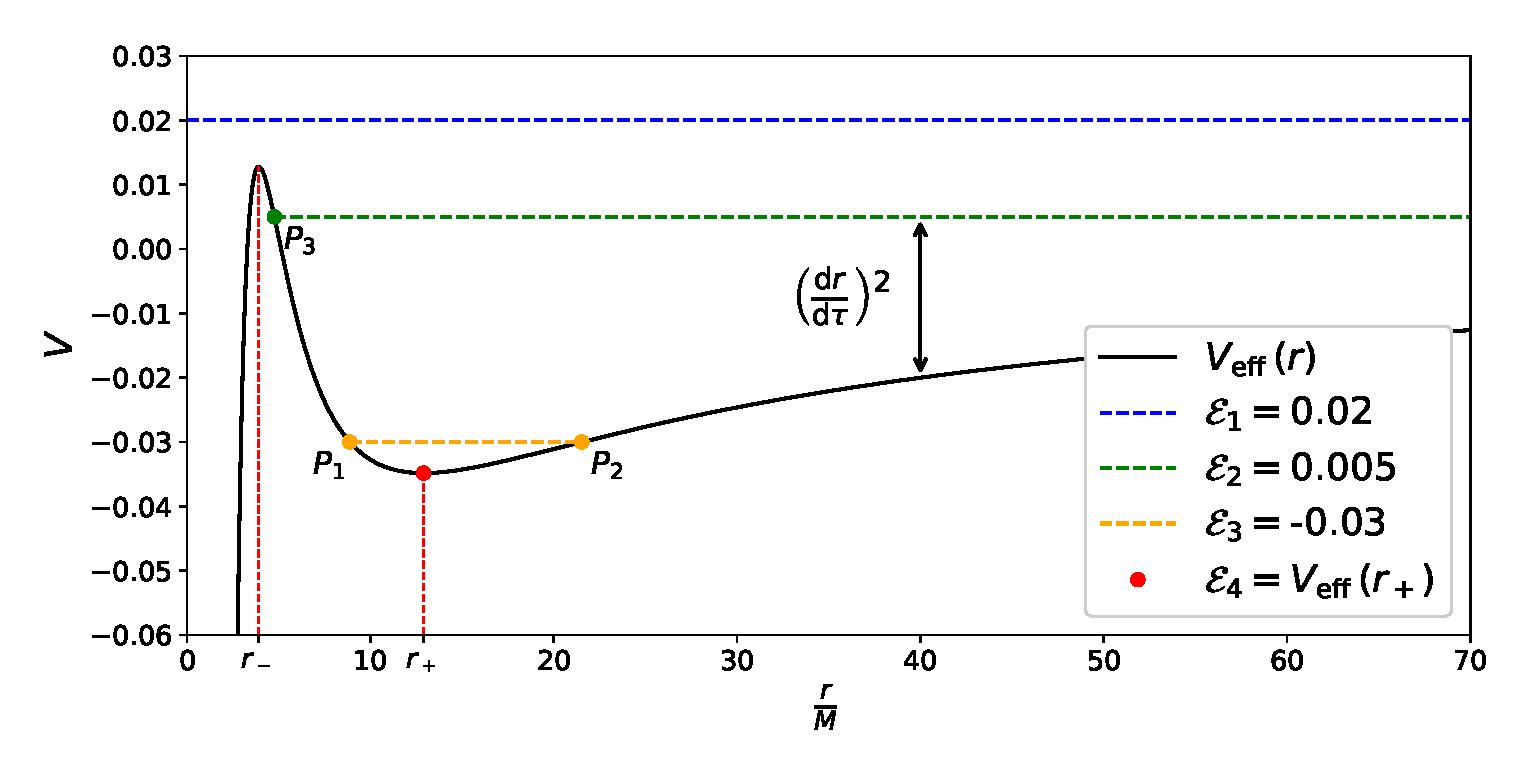
\includegraphics[width = \textwidth]{Figures/chapter1/V_eff_orbits.eps}
    \caption{In black the effective potential with $\ell / M = 4.1$.
    The dashed horizontal lines, along with the red dot, represent possible
    values of $\mathcal E$ that give 4 different scenarios.
    Refer to the text for a detailed explanation. \\
    \textit{This figure is inspired by
    \cite[page 245, Figure 12.2]{shapiro2008black}.}}
    \label{cap1:fig:V_eff_orbits}
\end{figure}

From eq. \ref{cap1:eq:like_newton} we know that the particle can change its
distance $r$ from the massive object only if there is the energy
$\mathcal E - V_{\rm eff}$ to do so.
In Figure \ref{cap1:fig:V_eff_orbits}, $V_{\rm eff}$ with $\ell / M = 4.1$ is
represented along with 4 different values of $\mathcal E$.

The red full dot represents the case where the particle has exactly the energy
required to stay in the local minimum of the potential.
Here there is no \textit{spare} energy that the particle can use to move along
$r$.
This is the case of a circular orbit, and it will be explored in Section
\ref{cap1:ssec:circular_orbits}

In the yellow case, $\mathcal E = -0.03$, the particle has some \textit{spare}
energy (not enough to escape) to change its radius between the two turning
points $P_1$ and $P_2$.
This results in an ellipse-like shape around the massive object.
\footnote{As we will see in Section \ref{cap1:sec:precession} it is not
exactly an ellipse as in the Newtonian case.}

Finally, the green case, $\mathcal E = 0.005$, and the blue one,
$\mathcal E = 0.02$, are not stable orbits.
In the first case, the particle has one turning point $P_3$ and has enough
energy to escape the potential well on the right and go back towards infinity.
In the latter, the particle as a bigger energy than $V_{\rm eff} (r_{\rm max})$
and can fall into the massive object, if $u^r$ is directed inward.


\subsection{Circular Orbits}
\label{cap1:ssec:circular_orbits}

As we have seen from Figure \ref{cap1:fig:V_eff_orbits} a particle can draw a
perfectly circular orbit if it has an energy $\mathcal E = V_{\rm eff}(r_{\rm min})$.
It is possible to find the relationship between the energy $e$
and angular momentum $\ell$ required that makes this possible and find a
general rule that describes the angular velocity of such orbits.

First of all, the four-velocity of the particle will be

\begin{equation}
    u^\mu = \left(\dv{t}{\tau}, 0, 0, \dv{\phi}{\tau} \right)
    = \left(\dv{t}{\tau}, 0, 0, \dv{t}{\tau} \Omega \right)
    = u^t (1, 0, 0, \Omega) \,
    \label{cap1:eq:circular_orbit_u}
\end{equation}

Where we defined $\Omega := \dv{\phi}{t}$: the rate at which $\phi$ changes with
respect to the \Sh time $t$.
Using eq. \ref{cap1:eq:conserved_e} and eq. \ref{cap1:eq:conserved_l}, $\Omega$
can be rewritten as

\begin{equation}
    \Omega := \dv{\phi}{t} = \dv{\tau}{t} \dv{\phi}{\tau} =
    \frac{1}{r^2} \left(1 - \frac{2M}{r} \right) \frac{\ell}{e}\, .
    \label{cap1:eq:Omega}
\end{equation}

A second equation for $\frac{\ell}{e}$ comes with the restriction that the
particle must orbit at the minimum of $V_{\rm eff}$, from eq.
\ref{cap1:eq:r_min_max}

\begin{equation}
    r = \frac{\ell^2}{2 M} \left[1 +
    \sqrt{1 - 12 \left( \frac{M}{\ell} \right)^2} \, \right] \, .
    \label{cap1:eq:r_min}
\end{equation}

Using eq. \ref{cap1:eq:found_e} the derivative of $r$ vanishes
and we can write everything as

\begin{equation}
    e^2 = \left(1 + \frac{\ell^2}{r^2} \right)
    \left(1 - \frac{2M}{r}\right) \, .
    \label{cap1:eq:circular_orbit1}
\end{equation}

Instead of substituting $r$ from eq. \ref{cap1:eq:r_min} into eq.
\ref{cap1:eq:circular_orbit1}, it is easier to solve eq. \ref{cap1:eq:r_min} for
$1 / \ell^2$ obtaining

\begin{equation}
    \frac{1}{\ell^2} = \frac{1}{M r} - \frac{3}{r^2} \, ,
\end{equation}

and then use it to rewrite eq. \ref{cap1:eq:circular_orbit1} as

\begin{align*}
    \frac{e^2}{\ell^2} &= \left(\frac{1}{\ell^2} + \frac{1}{r^2} \right)
    \left(1 - \frac{2M}{r}\right)
    %
    = \left(\frac{1}{M r}
    - \frac{3}{r^2}
    + \frac{1}{r^2}\right)
    \left(1 - \frac{2M}{r}\right) 
    %
    = \frac{1}{M r} \left(1
    - \frac{2 M}{r} \right)^2 \\
\end{align*}
\begin{equation}
    \frac{\ell}{e} = \sqrt{M r} \left(1
    - \frac{2 M}{r} \right)^{-1}
    \label{cap1:eq:circular_orbit2}
\end{equation}

We can finally substitute eq. \ref{cap1:eq:circular_orbit2} into eq.
\ref{cap1:eq:Omega} to get

\begin{equation}
    \Omega^2 = \frac{M}{r^3}
    \label{cap1:eq:Omega2}
\end{equation}

that gives the angular velocity observed from infinity of a particle in a
circular orbit.
With the value of $\Omega$ found in eq. \ref{cap1:eq:Omega2} we can find the
normalization of the four-velocity defined in \ref{cap1:eq:circular_orbit_u}.

\begin{align*}
    - 1 = \mathbf{u \cdot u} = g_{\nu \mu} u^\nu u^\mu
    &= (u^t)^2 \left[- \left(1 - \frac{2M}{r}\right) + r^2 \Omega^2 \right] \\
    (u^t)^2 &= \left[ 1 - \frac{2M}{r} - \frac{M}{r}\right]^{-1} \\
    u^t &= \left( 1 - \frac{3M}{r} \right)^{-1/2} \\
\end{align*}

Therefore, we have

\begin{equation}
    u^\mu = \left( 1 - \frac{3M}{r} \right)^{-1/2}
    \left( 1, 0, 0, \sqrt{\frac{M}{r^3}} \right)
\end{equation}


\subsection{General Shapes and Precession}
\label{cap1:sec:precession}

To complete the discussion on bound orbit we can have a look at a more general
case, where $V_{\rm eff} < \mathcal E < 0$.
If we want to characterize the shape of the orbit, as always restricted to the
$xy$ plane, we need to express $\phi$ as a function of $r$.
To do so we can use eq. \ref{cap1:eq:conserved_l} and eq. \ref{cap1:eq:found_e}
and rewrite them respectively as

\begin{subequations}
\begin{align}
    \dv{\phi}{\tau} &= \frac{\ell}{r^2} \label{cap1:eq:shape1} \\
    \dv{r}{\tau} &= \pm \sqrt{e^2 - \left(1 + \frac{\ell^2}{r^2}\right)
    \left(1 - \frac{2M}{r}\right)} \label{cap1:eq:shape2} \, .
\end{align}
\label{cap1:eq:to_find_shape}
\end{subequations}

This time we had no reason to keep one sign or the other in eq.
\ref{cap1:eq:shape2} as the radius can either increase or decrease.
Dividing \ref{cap1:eq:shape2} into \ref{cap1:eq:shape1} gives

\begin{equation}
    \dv{\phi}{r} = \pm \frac{\ell}{r^2}
    \left[e^2 - \left(1 + \frac{\ell^2}{r^2}\right)
    \left(1 - \frac{2M}{r}\right)\right]^{-1/2}
    \label{cap1:eq:shape}
\end{equation}

The function $\phi(r)$ can be found simply by integrating the right-hand side.
The result can be expressed in terms of elliptic functions but not in a very
enlightening way for those not familiar with them
\footcite[page 202]{hartle2021gravity}.

An interesting parameter to study is the \textit{precession}, defined as

\begin{equation}
    \delta \phi_{\rm prec} := \Delta \phi - 2 \pi
    \label{cap1:eq:precession}
\end{equation}

To define $\Delta \phi$ consider the turning points $P_1$ and $P_2$ in Figure
\ref{cap1:fig:V_eff_orbits}.
\textit{One orbit} is complete when the particle starts from the inner turning
point, $P_1$, and gets back to it.
We can equivalently consider $P_2$ as a starting and ending point.
$\Delta \phi$ is the angle swept during one orbit.
It's also useful to notice that the angle swept in one orbit is twice the angle
swept between $P_1$ and $P_2$, thus we can rewrite $\Delta \phi$ as

\begin{figure}[h]
    \centering
    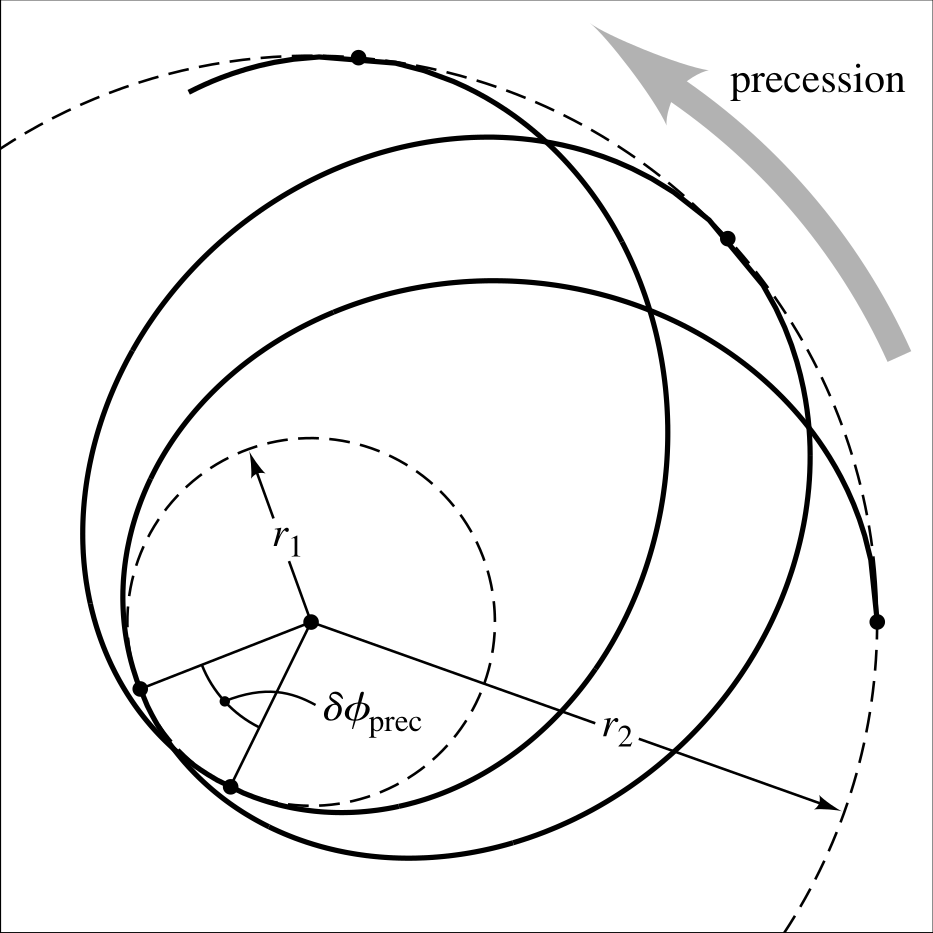
\includegraphics[width = 0.5 \textwidth]{Figures/chapter1/precession_bozza.png}
    \caption{Example of precession.
    Starting from an outer turning point one can trace the orbit ending up at
    different turning point, therefore sweeping an angle greater than $2 \pi$.
    \\ \fullcite[Figure 9.6, page 203]{hartle2021gravity}.}
    \label{cap1:fig:precession}
\end{figure}

\begin{equation}
    \Delta \phi = \int_{P_1}^{P_2} \dv{\phi}{r} \mathrm{d}r
    = 2 \ell \int_{r_1}^{r_2} \frac{1}{r^2}
    \left[e^2 - \left(1 + \frac{\ell^2}{r^2}\right)
    \left(1 - \frac{2M}{r}\right)\right]^{-1/2} \mathrm{d}r
    \label{cap1:eq:delta_phi}
\end{equation}

We used the positive solution from eq. \ref{cap1:eq:shape2} as we chose to
integrate from the inner turning point $P_1$ to the outer one $P_2$ that,
respectively correspond to a radius $r_1$ and $r_2$ where $r_1 < r_2$.
By the definition of the turning points, $r_1$ and $r_2$, the integral we need
to compute is between the two zeros of the denominator contained in square
brackets.
To check the correspondence with the Newtonian case we can solve the integral
in \ref{cap1:eq:delta_phi} neglecting the $r^{-3}$ term and remembering the
definition of $\mathcal E$ from eq. \ref{cap1:eq:found_epsilon}:

\begin{equation*}
    \Delta \phi = 2 \ell \int_{r_1}^{r_2} \frac{1}{r^2} \left[\mathcal E -
    \frac{\ell^2}{r^2}\ + \frac{2M}{r} \right]^{-1/2} \mathrm{d}r
\end{equation*}

Making the substitution $u = 1 / r$ and using the root of the denominator as
the bounds of integration we get

\begin{equation}
    \Delta \phi
    = 2 \int_{u_2}^{u_1} \frac{\mathrm{d} u}{\sqrt{(u_1 - u)(u - u_2)}} 
    = 2 \pi \quad \quad \forall u_1 \neq u_2
\end{equation}

where $u_{1/2} = \frac{1}{r_{1/2}}$.
The integral is $\pi$ for every $u_1$ and $u_2$, and therefore the precession
for an orbit predicted by Newtonian mechanics will always be $0$.

%% Problem 15 to get the expression in the first order of 1 / c^2 ?

\newpage


\section{Light Ray Orbits}

As we have introduced in eq. \ref{cap1:eq:u_light} and
\ref{cap1:eq:conserved_light}, the trajectory of a light ray, similarly to the
one of a massive particle, has the quantities $e$ and $\ell$ that are conserved.
We can therefore restrict the motion of the light ray to the $xy$ plane as we
did with massive particle and use $e$ and $\ell$ to write the four-velocity as

\begin{equation*}
    u^\mu
    = \left(\dv{t}{\lambda}, \, \dv{r}{\lambda}, \,
    0, \, \dv{\phi}{\lambda} \right)
    = \left( e \left(1 - \frac{2M}{r} \right)^{-1}, \, \dv{r}{\lambda}, \,
    0, \, \frac{\ell}{r^2} \right) \, .
\end{equation*}

The only difference lies, as described in eq.
\ref{cap1:eq:u_normalization_light}, in the normalization of $\mathbf u$, that
is $\mathbf{u \cdot u} = 0$.

So, with the same intent we had when we found eq. \ref{cap1:eq:found_e}, we can
write

\begin{equation*}
    0 = g_{\nu \mu} u^\nu u^\mu =
    - \left(1 - \frac{2M}{r} \right)^{-1} e^2
    + \left(1 - \frac{2M}{r} \right)^{- 1} \left(\dv{r}{\lambda} \right)^2
    + \frac{\ell^2}{r^2}
\end{equation*}

and then rearrange to get

\begin{equation}
    e^2 = \left( \dv{r}{\lambda} \right)^2 + \ell^2 \, W_{\rm eff} (r) \, .
    \label{cap1:eq:found_e_massless}
\end{equation}

Here we defined another effective potential, one that acts on light rays only,
as

\begin{equation}
    W_{\rm eff} (r) = \frac{1}{r^2} \left( 1 - \frac{2M}{r} \right) \, .
    \label{cap1:eq:W}
\end{equation}

\begin{figure}[h!]
    \centering
    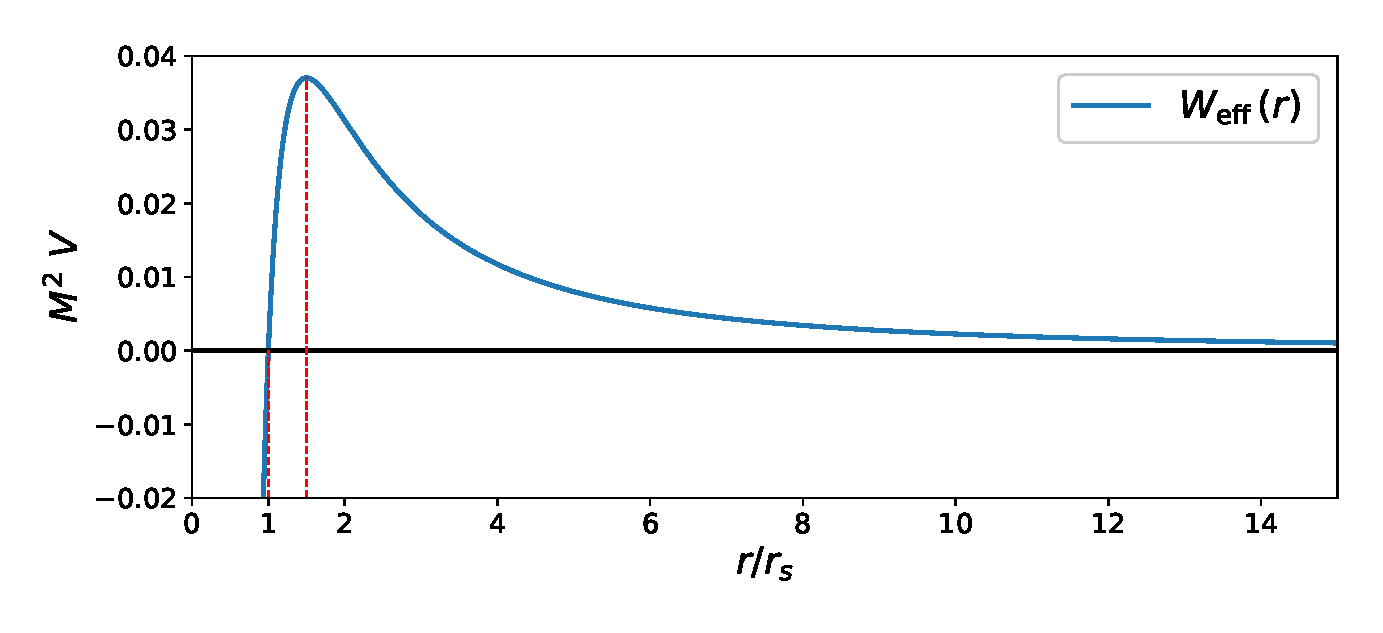
\includegraphics[width = 0.85 \textwidth]{Figures/chapter1/W_eff.eps}
    \caption{Effective potential for light rays, $W_{\rm eff}$, described in eq.
        \ref{cap1:eq:W}.
    We can see the maximum ar $r = 3M = 1.5 r_s$ and that the peak of
    $M^2 ~ W_{\rm eff}$ is at $1 / 27 \simeq 0.037$.}
    \label{ca1:fig:W_eff}
\end{figure}

This new potential can be studied, again, by taking the derivative of it with
respect to $r$.
We find out the there is one stationary point at $r = 3M$ representing
the maximum of the function, as we can also see from Figure \ref{ca1:fig:W_eff}.
This is therefore an unstable point, the value of the potential at the maximum
is

\begin{equation*}
    W_{\rm eff} (3 M) = \frac{1}{27 M^2} \, .
    \label{cap1:eq:max_W_eff}
\end{equation*}

It's interesting to notice that, unlike in the massive particle case, the
effective potential $W_{\rm eff}$ is independent of $l$.
Looking at eq. \ref{cap1:eq:found_e_massless} we can also rewrite it as

\begin{equation}
    \frac{1}{b^2} := \frac{e^2}{\ell^2}
    = \frac{1}{\ell^2} \left( \dv{r}{\lambda} \right)^2 + W_{\rm eff} (r) \, .
    \label{cap1:eq:found_b}
\end{equation}

where we defined $b = \abs{\ell / e}$.
Here we can use the fact the geodesic is invariant under an affine parameter
renormalization to ignore the $1 / \ell^2$ in front of the derivative of the
radius and understand that only the ratio $\frac{\ell}{e}$ holds
physical significance in the massless case.
%% devo aggiungere qualcosa? Una giustificazione?

To see what $b$ is, let's consider a particle approaching the massive object
from far away. In this case we will use Cartesian coordinates and say that the 
massive object is at the origin while the particle starts from a position
$(x, \, d)$, refer to figure \ref{cap1:fig:b}.

\begin{figure}[h]
\centering
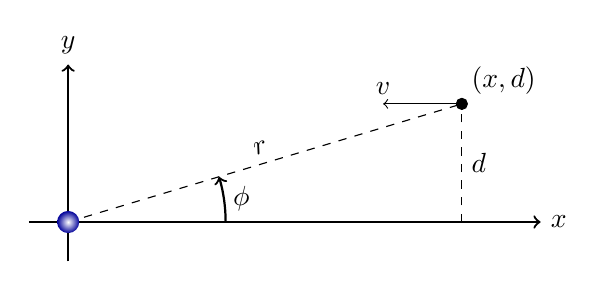
\begin{tikzpicture}

    % Cartesian axes
    \draw[thick,->] (-0.5,0) -- (6,0) node[right] {$x$};
    \draw[thick,->] (0,-0.5) -- (0,2) node[above] {$y$};

    % Particle at (x, d)
    \def\xP{5}
    \def\yP{1.5}
    \def\phiP{{atan(1.5 / 5)}}
    \filldraw[black] (\xP ,\yP) circle (2pt) node[anchor=south west] {$(x, d)$};

    % Draw the line r and d
    \draw[dashed] (0,0) -- (\xP, \yP) node[midway, above, sloped] {$r$};
    \draw[dashed] (\xP,0) -- (\xP, \yP) node[midway,right] {$d$};
    \draw[->] (\xP, \yP) -- (\xP - 1, \yP) node[above] {$v$};

    % Draw the angle theta
    \draw[thick,->] (2,0) arc [start angle=0,end angle=\phiP,radius=2cm];
    \node at (2.2,0.3) {$\phi$};

    % Star at origin (highlighted part)
    \shade[inner color=white, outer color=blue!60!black] (0,0,0) circle (4pt);

\end{tikzpicture}
\caption{Visual representation of a photon approaching the massive object
with an impact parameter $d$.}
\label{cap1:fig:b}
\end{figure}

If we evaluate $b$ in this scenario, considering $r \gg r_s$ and $r \gg d$, we
find out that

\begin{equation*}
    b = \abs{\frac{\ell}{e}}
    = \abs{r^2 \dv{\phi}{\lambda} \left(1-\frac{2M}{r}\right)^{-1}\dv{\lambda}{t}}
    \simeq \abs{r^2 \dv{\phi}{r}}
    \simeq \abs{r^2 \dv{}{r} \left(\frac{d}{r}\right)}
    = d \, . 
\end{equation*}

We can then interpret $b$ as the \textit{impact parameter} for a light ray at
infinity.

The shape of the orbit, determined by evaluating $\dv{r}{\lambda}$ from eq.
\ref{cap1:fig:b}, is therefore fully characterized by the value of $b$.

\begin{figure}[h!]
    \centering
    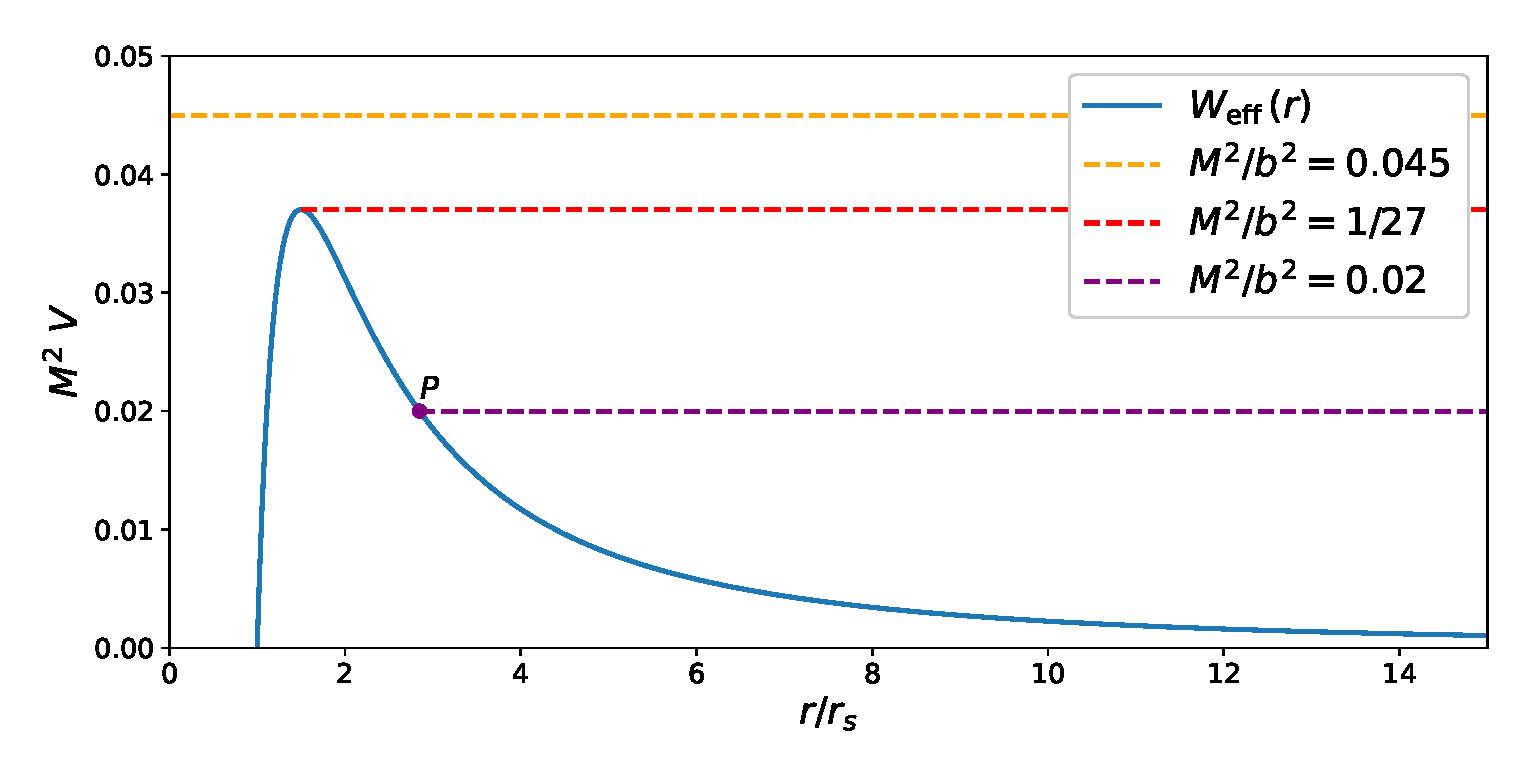
\includegraphics[width = 0.8 \textwidth]{Figures/chapter1/W_eff_vs_b.eps}
    \caption{Effective potential for light rays $W_{\rm eff}$, described in eq.
        \ref{cap1:eq:W}.
        Different values of the impact parameter $b$ give raise to 3 different
        type of orbits.}
    \label{ca1:fig:W_eff_orbits}
\end{figure}

Playing around with the possible values of $b$, because of the shape of
$W_{\rm eff}$, we can recognize 3 different types of orbits, that are shown in
Figure \ref{ca1:fig:W_eff_orbits}:

\begin{itemize}
    \item $b < 3 \sqrt{3} M$ (yellow dashed line): in this case the light ray
        doesn't have an impact parameter big enough and can surpass the
        potential barrier falling towards the center of the massive object;
    \item $b = 3 \sqrt{3} M$ (red dashed line): This represents an edge case 
        where the light ray can theoretically maintain a circular orbit at the
        unstable stationary point;
    \item $b > 3 \sqrt{3} M$ (purple dashed line): Here, the light ray has a
        sufficiently large impact parameter, allowing it to approach the massive
        object and, upon reaching the turning point $P$, continue its trajectory
        back to infinity.
        This results in a deflection of the light ray's path.

        
\end{itemize}

%% Section with expample 9.2?


\section{Deflection of Light}

The phenomenon of light deflection, briefly mentioned earlier, is particularly
interesting in terms of measurable effects.
This effect is, for example, visible in distant stars whose light is deflected
by the sun and then observed from the earth.

To find the deflection it is useful to first express $\phi$ as a function of
$r$.
We can rewrite eq. \ref{cap1:eq:e_light} and eq. \ref{cap1:eq:found_b} as

\begin{subequations}
\begin{align}
    \frac{1}{\ell} \dv{\phi}{\lambda} &= \frac{1}{r^2}
    \label{cap1:eq:phi_of_lambda} \\
    \frac{1}{\ell} \dv{r}{\lambda} &= \sqrt{\frac{1}{b^2} - W_{\rm eff}}
    \label{cap1:eq:r_of_lambda} \, .
\end{align}
\end{subequations}

Dividing eq. \ref{cap1:eq:r_of_lambda} into \ref{cap1:eq:phi_of_lambda} and
recalling the complete expression of $W_{\rm eff}$ from eq. \ref{cap1:eq:W} we
get

\begin{equation}
    \dv{\phi}{r} = \frac{1}{r^2} \left[\frac{1}{b^2}
    - \frac{1}{r^2} \left(1 - \frac{2M}{r} \right) \right]^{-1/2} \, .
    \label{cap1:eq:phi_of_r_light}
\end{equation}

Looking at Figure \ref{cap1:fig:deflection} we can see the deflected ray in
thick dashed line spanning an angle $\Delta \phi$ (if we consider it coming from
infinity and going back to infinity).
A non-deflected ray on the other hand will span an angle of $\pi$.
The deflection angle we are interested in is therefore the one labeled as
$\delta \phi_{\rm def}$ and is calculated by doing

\begin{equation}
    \delta \phi_{\rm def} = \Delta \phi - \pi
    \label{cap1:eq:delta_Delta}
\end{equation}

In the Figure \ref{cap1:fig:deflection}, $r_1$ represents the turning point, the
point where the light is closer to the massive object (refer to Figure
\ref{ca1:fig:W_eff_orbits}).
Most importantly in this case, $r_1$ cuts the trajectory in half.
We can then evaluate half the angle angle spanned by integrating eq.
\ref{cap1:eq:phi_of_r_light} from $r = r_1$ to $r = \infty$.
Consequently, the full angle spanned by the deflected light ray will be

\begin{equation}
    \Delta \phi = 2\int_{r_1}^\infty \frac{1}{r^2} \left[\frac{1}{b^2}
    - \frac{1}{r^2} \left(1 - \frac{2M}{r} \right) \right]^{-1/2} \mathrm{d}r
    \label{cap1:eq:deflection}
\end{equation}

remembering from Figure \ref{ca1:fig:W_eff_orbits} that $r_1$ is measured when
the light ray is in $P$ and $1 / b^2 = W_{\rm eff}(r_1)$

\begin{figure}[h]
    \centering
    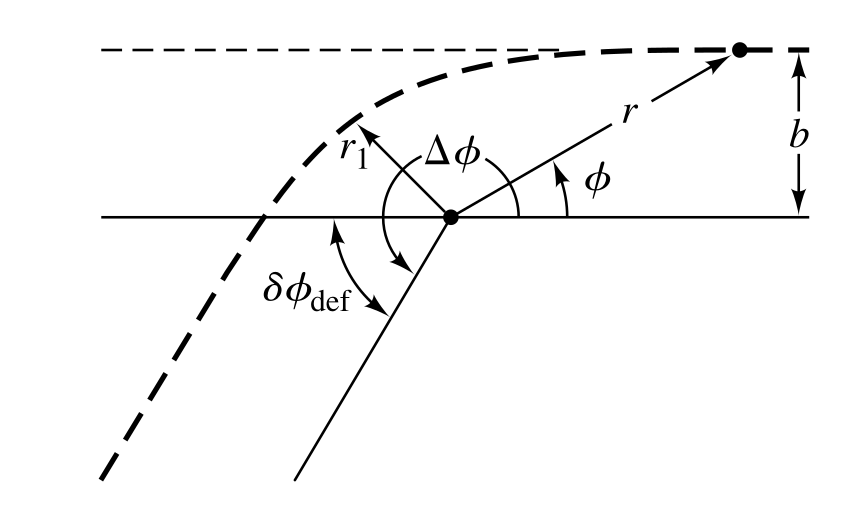
\includegraphics[width = 0.5 \textwidth]{Figures/chapter1/deflection.png}
    \caption{Deflected ray, in a thick dashed line, against the non-deflected
    trajectory, in thin dashed line.
    A non-deflected ray that goes from right to left (infinitely far) would span
    an angle of $\pi$.
    The deflected ray instead spans an angle of $\Delta \phi$. \\
    \textit{From} \cite{hartle2021gravity} \textit{page 211, Figure 9.10}}
    \label{cap1:fig:deflection}
\end{figure}

In the integral in \ref{cap1:eq:deflection} we can make the substitution
$w = b / r$ to rewrite it as

\begin{equation}
    \Delta \phi = 2 \int_o^{w_1}
    \left[1 - w^2 \left(1 - \frac{2M}{b}w\right)\right]^{-1/2} \mathrm{d}w
    \label{cap1:eq:deflection_w}
\end{equation}

where $w_1$ is the value at which the square bracket vanishes.
Using eq. \ref{cap1:eq:delta_Delta} and eq. \ref{cap1:fig:deflection_w} we can
numerically evaluate the integral for different values of $b$.
The result is shown in Figure \ref{cap1:fig:deflection_w}.

\begin{figure}[h]
    \centering
    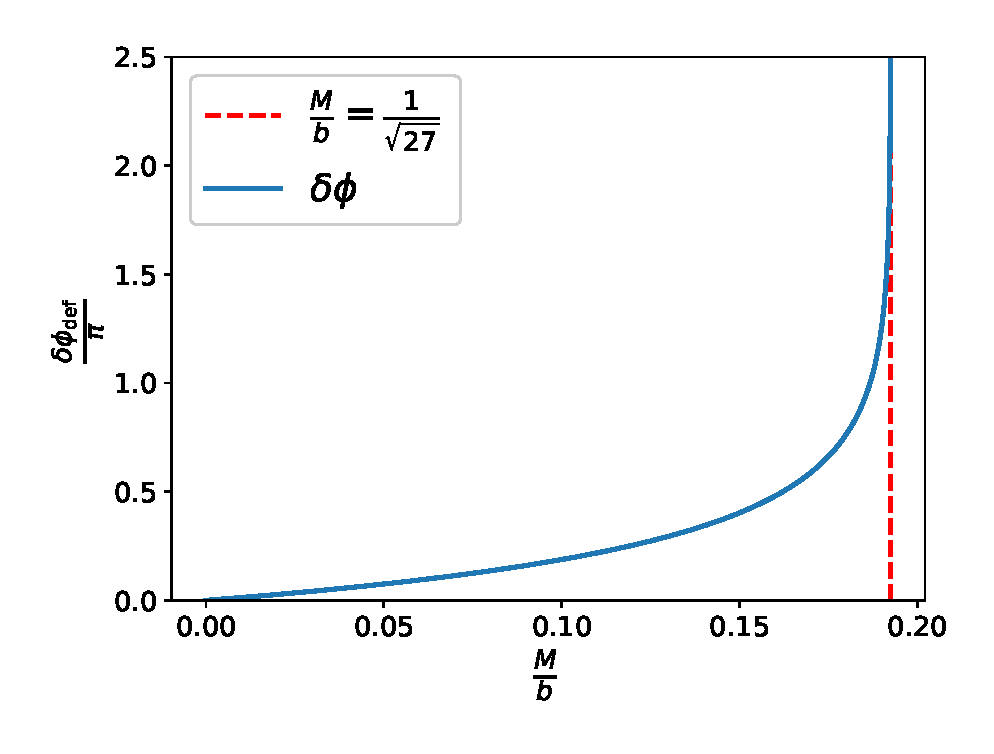
\includegraphics[width = 0.65 \textwidth]{Figures/chapter1/deflection_w.eps}
    \caption{Deflection of a light ray because of the gravitational field of a
    massive object.
    As $1 / b^2 \rightarrow 27 M^2$ the light ray trajectory gets closer to a
    circular orbit, and the ray can turn around the massive object multiple
    times before going back to infinity.}
    \label{cap1:fig:deflection_w}
\end{figure}


